\section{FairTest}
\label{sect:fairtest}

\begin{figure}[h]
 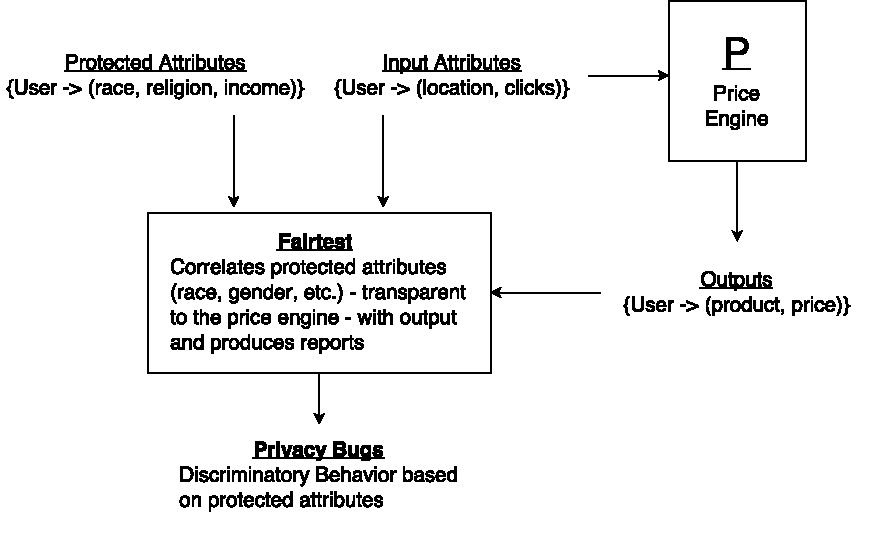
\includegraphics[width=0.49\textwidth]
  {\detokenize{figures/overview}}
  \caption{ {\bf \textit{FairTest} use overview}. Gives an overview of how an application
    may use \sysname to generate bug-reports.
  }
  \label{fig:FairtestOverview}
\end{figure}

In this section we present the design and implementation of \sysname.
At its core, \sysname assets that there are no violations of
{\em statistical parity} (condition~\ref{eq:StatisticalParity}
- Section~\ref{sect:statparity}).
Figure~\ref{fig:FairtestOverview}, gives an overview of how a data-driven
application with a pricing policy ``P'' can use \sysname to generate
bug reports. As shown in Figure~\ref{fig:FairtestOverview}, user-attributes
(protected and non-protected) and price engine's outputs are used by
\sysname to generate bug-reports. \sysname generates these report based on
the {\em statistical parity} of users on certain protected attributes
(such as gender, race, etc.). Any violation of
condition~\ref{eq:StatisticalParity}, is reported by \sysname as a {\em privacy bug}.

\sysname is designed to be used both by developers and by auditors of
data-driven web applications. It is interfaced with REST API that can be
used by web applications, without any fundamental limitation.
We expect developers to make only minimal modifications to their
application (mostly adding the tracking code) in order to provide
\sysname with the data necessary for auditing. To address privacy on the
testing framework, \sysname does not require identifiable user information,
such as exact address, name, etc. The framework itself is implemented in
the Django Python web framework with an SQLite database.

\sysname can generate bug-reports for registered users by asserting
{\em statistical parity} of users. The reports are accessible either
through \sysname's RESTful API or its web interface.
With the information, a developer or an auditor can then identify potential
\textit{privacy bugs} that are caused by the statistical parity violations
customization engine appears acceptable or not.
In what follows we present the architecture and the API of our \sysname
implementation.

\subsection{Architecture}
Our \sysname implementation consists of three parts:
(i) a REST API that gathers data from monitored application;
(ii) a statistical engine that asserts statistical parity between protected
user attributes;
and (iii) a reporting tool that generates bug-reports.
Figure~\ref{fig:FairtestArch} demonstrates this architecture and a sample workflow.
The input API receives requests from the monitored
application and records all inputs and outputs regarding a user.
At the same time, \sysname accepts queries for bug-reports with respect
to certain protected attributes.

\begin{figure}[h]
 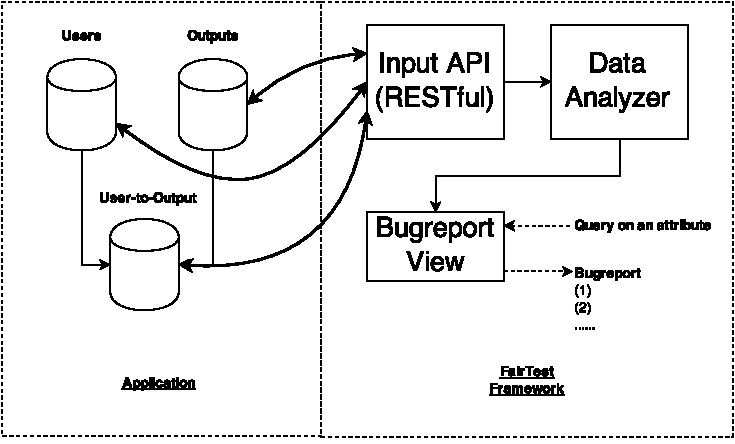
\includegraphics[width=0.49\textwidth]
  {\detokenize{figures/architecture}}
  \caption{{\bf \textit{FairTest}'s architecture}. The diagram shows \sysname's architecture,
    along with a very simple application using it. Bold lines represent API
    calls and dash lines represent bug-report queries. Solid line indicate data flow
    as part of the application or of the testing framework.}
  \label{fig:FairtestArch}
\end{figure}

\subsection{API}
\begin{table}[t]
{
 \scriptsize
  \renewcommand{\arraystretch}{1.5}
  \begin{tabular}{ l | l }
    Usage & Function \\
    \hline
    POST /user & Add a user with attributes \\
    POST /output & Add a output from the program \\
    POST /user/12/output & Link an output to a user\\
    \hline
    PUT /user/12 & Change attributes of user \#12 \\
    \hline
    GET /user/12 & Get information of user \#12 \\
    GET /user/12/output & Get outputs for user \#12 \\
  \end{tabular}
  \caption{{{\bf \textit{FairTest}'s API}}. Summarizes \sysname's
      REST API.}
  \label{tab:fairtestApi}
}
\end{table}


\textit{FairTest} incorporates a REST API for gathering data from the
application and generating bug-reports. Its basic functions are summarized
in Table~\ref{tab:fairtestApi}.

As can be seen, this API contains very simple operations to be linked into
the application. As a RESTful API, it also has support in most programming
languages to add the outputs directly from the MVC models. It also offers
a simple querying mechanism for the developer to check validity of data.

As the data model is simple, we expect this API to be scalable as well.
